
\section{The Storybook}
The storybook contains all of the stories you can play in Wheel of Elements.
Each story will take about 2.5 hours to play through. One session includes 3 encounters and one text containing a short story explaining your cause and circumstance.

\begin{figure}[ht]
	\begin{minipage}[t][9cm][t]{0.5\textwidth}
		\begin{minipage}[t][5cm][t]{0.9\textwidth}
			\fbox{\parbox[4cm]{\textwidth}{Picture:  Storybook}}
		\end{minipage}
	\end{minipage}
	\begin{minipage}[t][9cm][t]{\textwidth}
		
		\subsection*{Stories}
		Each story begins with an introduction, which should be narrated by a player.
		The text is separated into four sections. After reading a section, start the \textbf{fight} below that story section. After finishing a fight, read the next story section, draw an \textbf{event}  \textit{See Section Events, Page \pageref{Section_Events}} and \textbf{level up} \textit{See Character Building, Page \pageref{Section_CharacterBuilding}}. Repeat this process after finishing the second encounter.
		%Flowchart? with nice pics?
		
		
		\subsection*{Encounters}
		Each story comes with three enemy encounters. An encounter presents which enemies should be fought and in which arrangement.
		There are always \textbf{5 enemy setups} described per encounter. Each player takes one setup, matching the seating order.
		These enemy setups are \textbf{distributed clockwise} by seating order. %Please get  a picture for this
		If you are playing with less than 5 players, ignore the setups beyond your player number.
		After the first and second encounter, you level up. \textit{See Character Building, Page \pageref{Section_CharacterBuilding}}
		
	\end{minipage}	
	
	%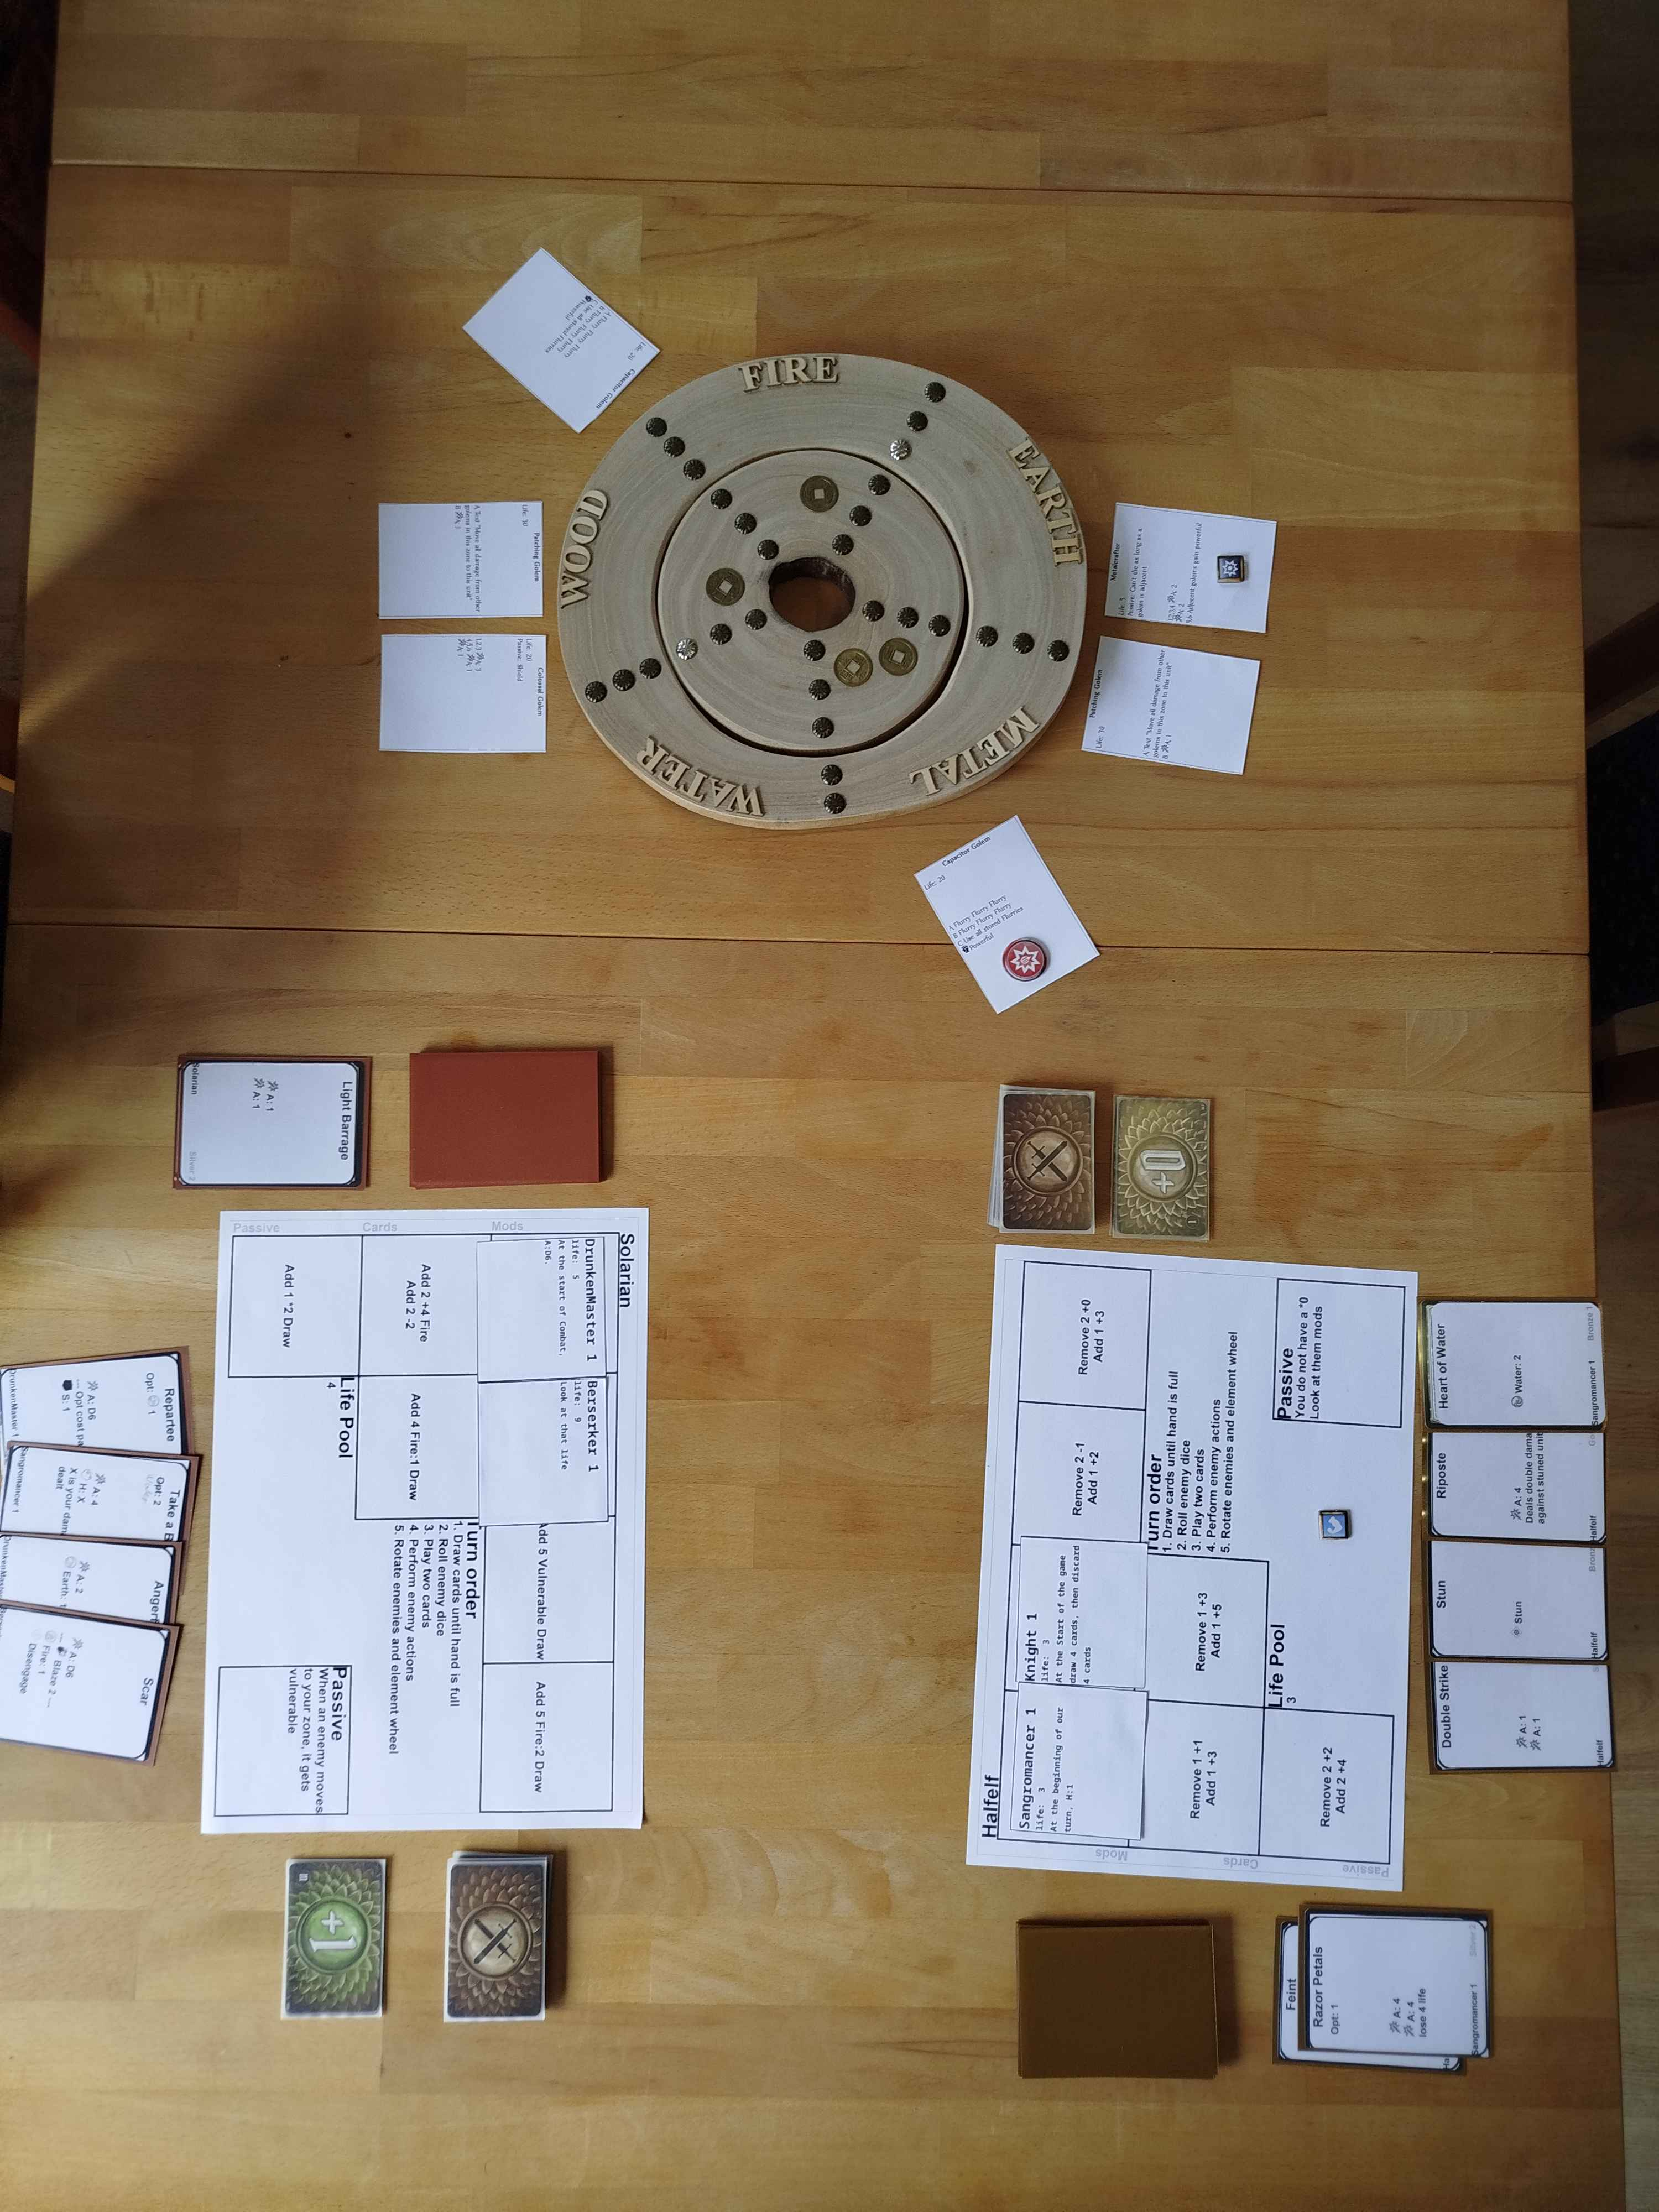
\includegraphics[width=0.8\textwidth]{../ExplanationPics/TwoBoards.jpg}
\end{figure}



\fbox{\parbox[4cm]{\textwidth}{Picture:  Dragon flying overhead of some Solarians/Wyrmlings}}